\chapter{Robotic arms and direct kinematics}
\label{chap:lecture10}

A mobile robot can often be modeled as one rigid body moving through the
world. A robotic arm instead consists of several rigid bodies whose relative
poses change at joints. Its configuration must describe those internal
motions as well as the resulting position and orientation of its tool.
The coordinate transformations developed earlier provide a systematic way
to connect joint variables to tool pose.

\section{Links, joints, and the end effector}
The individual rigid bodies of a manipulator are called \emph{links}.
\emph{Joints} connect adjacent links and constrain their relative motion.
A sequence of links and joints forms a \emph{kinematic chain}. Here we
consider a serial, open chain with a fixed base: there is one path from
the base to the terminal link, with no closed loops.

Number the base as link 0 and the moving links as $1,\ldots,n$.
Joint $i$ connects link $i-1$ to link $i$. The terminal tool is the
\emph{end effector}: it may be a gripper, welding tool, drill, or another
device selected for the task. A tool rigidly attached to the last link is
part of that link for the arm's kinematic model. Additional tool motions,
such as opening gripper fingers, require extra coordinates if they are
included in the model.

\subsection{Revolute and prismatic joints}
Two common one-degree-of-freedom joints are:
\begin{itemize}
\item A \emph{revolute} or rotational joint, denoted R, permits relative
rotation about an axis. Its joint variable is an angle, typically measured
in radians.
\item A \emph{prismatic} joint, denoted P, permits relative translation
along an axis. Its joint variable is a displacement, typically measured
in meters.
\end{itemize}
These names describe the joints, not the rigid links themselves. In a
schematic, a cylinder can indicate a revolute joint with its axis along
the cylinder's length. A sliding block can indicate a prismatic joint,
but its translation direction must also be shown.

\begin{figure}[htbp]
\centering\begin{tikzpicture}
\draw[very thick,gray] (0,-1)--(0,-.5);
\draw[fill=gray!15] (-.45,-.5)--(-.45,.65) arc (180:360:.45 and .16)--(.45,-.5);
\draw (-.45,-.5) arc (180:360:.45 and .16);
\draw[fill=gray!15] (0,.65) ellipse (.45 and .16);
\draw[very thick,gray] (0,.8)--(0,1.4)--(1.5,1.4);
\draw[projection] (0,-1.15)--(0,1.8);
\draw[axis,robotframe] (.65,-.3) arc (0:280:.65 and .25);
\node[robotframe,right] at (.75,-.2) {$q_i$};
\node at (.5,-1.7) {Revolute (R)};
\begin{scope}[shift={(6,0)}]
\draw[very thick,gray] (-1.5,0)--(1.7,0);
\draw[fill=gray!15] (-.6,-.35) rectangle (.6,.35);
\draw[very thick,gray] (0,.35)--(0,1.4)--(1.5,1.4);
\draw[<->,thick,sensorframe] (-.8,-.85)--node[below]{$q_i$}(.8,-.85);
\node at (.2,-1.7) {Prismatic (P)};
\end{scope}
\end{tikzpicture}

\caption{Symbols for one-degree-of-freedom joints. The revolute coordinate
measures relative rotation; the prismatic coordinate measures relative
translation. Joint zero positions and positive directions are part of the
model definition.}
\label{fig:l10-joints}
\end{figure}

A chain described as RRRRP has four revolute joints followed by one
prismatic joint. This sequence alone does not determine its geometry:
the axes' positions and directions, the distances between joints, and
the tool attachment are also needed. Two joint axes that appear parallel
in one configuration need not remain parallel when an intervening joint
rotates.

\section{Joint variables and degrees of freedom}
An unconstrained rigid body in space has six degrees of freedom: three
for translation and three for orientation. Five independent free bodies
would therefore have 30 degrees of freedom. Connecting those bodies into
a fixed-base serial chain changes the count because the joints constrain
their relative motion.

For an open chain of $n$ independent one-degree-of-freedom joints, its
configuration can be specified by
\begin{equation}
 q=\begin{bmatrix}q_1&q_2&\cdots&q_n\end{bmatrix}\trans.
 \label{eq:l10-q}
\end{equation}
Thus the RRRRP chain has five configuration degrees of freedom. Its first
four coordinates are angles and its last coordinate is a displacement.
The components of a joint vector need not all have the same units.

This count assumes the stated open-chain structure and independent joints.
Couplings, closed loops, a moving base, or multi-degree-of-freedom joints
require a different count. Joint limits restrict the allowable range of
each coordinate. An angle may be periodic for a freely rotating joint,
but a physical joint need not allow unlimited rotation.

In a purely kinematic description, $q$ is often called the state. For a
dynamic model that predicts motion from torques or forces, position alone
is generally insufficient; joint velocities are also needed.

\begin{figure}[htbp]
\centering\begin{tikzpicture}[x=1cm,y=1cm]
\draw[thick] (-.3,-.5)--(-.3,.5);
\foreach \y in {-.4,-.2,0,.2,.4} {\draw (-.5,\y-.1)--(-.3,\y);}
\draw[very thick,gray] (-.3,0)--(10.5,0);
\foreach \i/\x in {1/.6,2/2.6,3/4.6,4/6.6} {
 \node[draw,circle,fill=white,minimum size=.55cm] at (\x,0) {R};
 \node[above] at (\x,.4) {$J_{\i}$};
 \node[robotframe,below] at (\x,-.4) {$q_{\i}$};
}
\node[draw,fill=white,minimum size=.55cm] at (8.6,0) {P};
\node[above] at (8.6,.4) {$J_5$};
\node[sensorframe,below] at (8.6,-.4) {$q_5$};
\foreach \i/\x in {1/1.6,2/3.6,3/5.6,4/7.6,5/9.6} {
 \node[above] at (\x,0) {link \i};
}
\draw[thick] (10.5,-.35)--(10.5,.35)--(11,.35);
\draw[thick] (10.5,-.35)--(11,-.35);
\node[below] at (10.6,-.55) {EE};
\node[below,align=center] at (-.45,-.65) {base\\link 0};
\end{tikzpicture}

\caption{Topology of a five-joint RRRRP chain. Joint $i$ connects links
$i-1$ and $i$. The drawing identifies connectivity and coordinate dependence;
it does not prescribe the spatial directions of the joint axes.}
\label{fig:l10-chain}
\end{figure}

\section{Direct and inverse kinematics}
Attach a frame to the end effector and denote it by EE. The
\emph{direct kinematics}, also called \emph{forward kinematics}, maps the
joint configuration to the end-effector pose:
\begin{equation}
 q\longmapsto H_{\mathrm{EE}}^W(q)
 =\begin{bmatrix}
 R_{\mathrm{EE}}^W(q)&p_{\mathrm{EE}}^W(q)\\
 0\;0\;0&1
 \end{bmatrix}.
 \label{eq:l10-direct}
\end{equation}
The joint coordinates might be measured by encoders. The result states
where the tool is and how it is oriented in the world frame.

Using roll, pitch, and yaw to describe orientation, one can also express
the output locally as six scalar functions:
\[
 \begin{bmatrix}x_{\mathrm{EE}}^W\\y_{\mathrm{EE}}^W\\z_{\mathrm{EE}}^W\\
 \varphi_{\mathrm{EE}}^W\\\theta_{\mathrm{EE}}^W\\\psi_{\mathrm{EE}}^W
 \end{bmatrix}
 =\begin{bmatrix}f_1(q)\\f_2(q)\\f_3(q)\\f_4(q)\\f_5(q)\\f_6(q)\end{bmatrix}.
\]
The homogeneous matrix is often the more convenient output because it
avoids choosing among multiple angle representations. For a specified
rigid serial-chain geometry and a given admissible $q$, the physical tool
pose is unique. Different roll--pitch--yaw triples can nevertheless represent
the same orientation, and angle extraction has singular cases.

\subsection{The inverse question}
Suppose a sensor detects an object and its pose has been expressed in the
world frame. To grasp it, the robot needs joint coordinates that place its
tool at a desired pose. This is \emph{inverse kinematics}:
\begin{equation}
 \text{given }H_{\mathrm{EE},d}^W,\qquad
 \text{find }q\text{ such that }H_{\mathrm{EE}}^W(q)=H_{\mathrm{EE},d}^W.
 \label{eq:l10-inverse}
\end{equation}
The desired tool frame may have a known offset from the object frame;
their origins and axes do not have to coincide for a grasp to be correct.

Forward kinematics evaluates a function. Inverse kinematics solves
equations, usually nonlinear ones. Depending on the geometry, target,
and constraints, there may be no solution, one solution, several isolated
solutions, or infinitely many solutions. A general closed-form inverse
need not be available, even when the forward model is explicit.

The inverse-kinematics problem is not the same as inverting a homogeneous
matrix. $(H_{\mathrm{EE}}^W)^{-1}$ expresses the world frame relative to
the end effector for an already known pose; it does not recover the joint
coordinates that produce that pose.

\section{Building direct kinematics from local transformations}
Place a frame $i$ rigidly on each link $i$. For now, take the base frame 0
to coincide with the world frame. The essential observation is that the
relative pose of adjacent link frames depends only on their connecting
joint coordinate and the fixed geometry:
\begin{equation}
 H_i^{i-1}=H_i^{i-1}(q_i).
 \label{eq:l10-local}
\end{equation}
For example, if joint 2 remains fixed while joint 1 moves, links 1 and 2
move together. Their world poses change, but $H_2^1$ does not. Moving a
joint farther along the chain likewise does not alter the relative pose
of links 1 and 2. Moving joint 2 itself does change $H_2^1$.

The local transformations compose in the same order as the coordinate
transformations studied earlier:
\begin{equation}
 \boxed{H_n^0(q)=H_1^0(q_1)H_2^1(q_2)\cdots H_n^{n-1}(q_n).}
 \label{eq:l10-product}
\end{equation}
For the five-joint chain,
\[
 H_5^0=H_1^0H_2^1H_3^2H_4^3H_5^4
 =\begin{bmatrix}R_5^0&p_5^0\\0\;0\;0&1\end{bmatrix}.
\]
Each factor maps coordinates from its subscript frame to its superscript
frame. Applied to a point in frame 5, the rightmost factor acts first.
The matching intermediate frame labels help verify the order; in general
the factors cannot be reordered.

The same idea also gives the pose of an intermediate link:
$H_i^0=H_1^0\cdots H_i^{i-1}$. This world-relative pose depends on the
preceding joint coordinates, even though each adjacent-frame factor
depends on only one coordinate.

\subsection{Base and tool offsets}
If the base does not coincide with the world frame, include its mounting
transform. If the tool frame does not coincide with frame $n$, include the
tool attachment transform:
\begin{equation}
 H_{\mathrm{EE}}^W
 =H_0^W\left(H_1^0\cdots H_n^{n-1}\right)H_{\mathrm{EE}}^n.
 \label{eq:l10-offsets}
\end{equation}
For a fixed base and a rigidly mounted tool, the outer two factors are
constant. Thus the full problem separates into local joint transformations
and fixed geometric offsets.

The remaining task is to choose frames and construct each local matrix
systematically. Standard frame-assignment conventions make that process
repeatable. Before introducing such a convention, a planar arm provides
a case simple enough to derive directly from geometry.

\section{A planar two-link manipulator}
Consider two revolute joints and two links of lengths $\ell_1,\ell_2>0$,
moving in the world $xy$ plane. The first joint is at the world origin.
Let $q_1$ be the first link's angle from $x_W$, and let $q_2$ be the second
link's angle \emph{relative to the first link}. Both angles are positive
counterclockwise.

Place the end-effector frame 2 at the tip, with $x_2$ along the second link
and $y_2$ perpendicular to it in the plane. The second link's world
orientation is $q_1+q_2$, not $q_2$ alone.

\begin{figure}[htbp]
\centering\begin{tikzpicture}[scale=1.05]
\coordinate (O) at (0,0);
\coordinate (A) at (2.598,1.5);
\coordinate (B) at (3.177,3.092);
\draw[axis] (-.4,0)--(5,0) node[right] {$x_W=x_0$};
\draw[axis] (0,-.3)--(0,4) node[above] {$y_W=y_0$};
\draw[very thick] (O)--node[above,sloped] {$\ell_1$}(A)--node[above,sloped] {$\ell_2$}(B);
\foreach \p in {O,A} {\draw[fill=white,thick] (\p) circle (.11);}
\fill (B) circle (.045);
\draw[projection] (A)--(2.598,0);
\draw[projection] (A)--(3.8,1.5);
\draw[projection] (B)--(3.177,0);
\draw[projection] (B)--(0,3.092);
\draw[projection] (A)--++(30:1.5);
\draw[axis,robotframe] (.8,0) arc (0:30:.8);
\node[robotframe] at (1,.24) {$q_1$};
\draw[axis,robotframe] ($(A)+(30:.8)$) arc (30:70:.8);
\node[robotframe] at ($(A)+(47:1.12)$) {$q_2$};
\draw[axis,sensorframe] (B)--++(70:1) node[above] {$x_2$};
\draw[axis,sensorframe] (B)--++(160:1) node[left] {$y_2$};
\node[below] at (3.177,0) {$x_2^W$};
\node[left] at (0,3.092) {$y_2^W$};
\node[below left] at (O) {$O_0$};
\end{tikzpicture}

\caption{A planar RR arm. The second joint angle is measured from the
extension of the first link. Dashed projections separate the two link
contributions to the end-effector position.}
\label{fig:l10-planar}
\end{figure}

Adding the two link vectors gives
\begin{equation}
 \boxed{\begin{aligned}
 x_2^W&=\ell_1\cos q_1+\ell_2\cos(q_1+q_2),\\
 y_2^W&=\ell_1\sin q_1+\ell_2\sin(q_1+q_2),\\
 \psi_2^W&=q_1+q_2.
 \end{aligned}}
 \label{eq:l10-planar}
\end{equation}
With the frame axes chosen as stated, $z_2^W=0$ and roll and pitch can
both be taken as zero. The yaw is understood modulo $2\pi$ when it
represents orientation rather than accumulated joint rotation.

\subsection{Recovering the same result by matrix multiplication}
Place frame 1 at the elbow, rigidly attached to link 1, with $x_1$ along
that link. In planar homogeneous coordinates,
\begin{align}
 H_1^0(q_1)&=\begin{bmatrix}
 \cos q_1&-\sin q_1&\ell_1\cos q_1\\
 \sin q_1&\cos q_1&\ell_1\sin q_1\\0&0&1
 \end{bmatrix},\\
 H_2^1(q_2)&=\begin{bmatrix}
 \cos q_2&-\sin q_2&\ell_2\cos q_2\\
 \sin q_2&\cos q_2&\ell_2\sin q_2\\0&0&1
 \end{bmatrix}.
\end{align}
Multiplying them produces
\begin{equation}
 H_2^0=\begin{bmatrix}
 \cos(q_1+q_2)&-\sin(q_1+q_2)&x_2^W\\
 \sin(q_1+q_2)&\cos(q_1+q_2)&y_2^W\\
 0&0&1
 \end{bmatrix},
 \label{eq:l10-planarmatrix}
\end{equation}
where the translation entries agree with Equation~\eqref{eq:l10-planar}.
These are $3\times3$ planar transformations. The corresponding spatial
matrix is $4\times4$, with a $z$ rotation, zero $z$ translation, and the
usual homogeneous last row.

\subsection{Worked example}
Let $\ell_1=1\,\mathrm m$, $\ell_2=0.5\,\mathrm m$,
$q_1=\pi/6$, and $q_2=\pi/3$. The second link is vertical because
$q_1+q_2=\pi/2$. Therefore
\[
 x_2^W=\frac{\sqrt3}{2}\,\mathrm m,\qquad
 y_2^W=\left(\frac12+\frac12\right)\mathrm m=1\,\mathrm m,
 \qquad\psi_2^W=\frac\pi2.
\]
The planar pose matrix is
\[
 H_2^0=\begin{bmatrix}0&-1&\sqrt3/2\\1&0&1\\0&0&1\end{bmatrix}.
\]
The matrix and geometric constructions describe the same tool pose.

\section{Task dimension, reachability, and redundancy}
The planar RR arm has two independent joint coordinates. A full planar
tool pose has three components $(x,y,\psi)$, so the arm cannot generally
set all three independently. Specifying a reachable position can determine
one or more joint configurations, each with an associated orientation;
there is not generally a freely selectable yaw left over.

This is a limitation relative to the chosen task. If both joints have
independent actuators, the arm is \emph{fully actuated in joint space}.
Having too few configuration degrees of freedom for an arbitrary task
pose is different from \emph{underactuation}, which concerns having fewer
independent actuation inputs than configuration degrees of freedom.

A planar three-revolute-joint chain can generally control a full planar
pose locally away from singular configurations. A planar chain with more
than three independent joints is typically \emph{kinematically redundant}
for that task: different joint configurations can produce the same tool
pose. This extra freedom can allow internal motion while the tool remains
fixed, subject to joint limits, collisions, and the particular configuration.
For a position-only task, even a three-joint planar arm can be redundant.
Redundancy is therefore defined relative to the task, not by counting
motors alone.\footnote{For terminology and inverse-kinematics context, see
Lynch and Park, \href{https://modernrobotics.northwestern.edu/nu-gm-book-resource/inverse-kinematics-of-open-chains/}{Modern Robotics, Chapter 6}.}

Counting degrees of freedom is a useful first check, but is not a guarantee
that a target can be reached. Geometry, joint limits, and singular
configurations still matter even when the number of joints matches the
number of task coordinates.

\subsection{Position workspace of the two-link arm}
With unrestricted revolute joints and no collision constraints, the
distance $\rho$ of the tip from the base satisfies
\begin{equation}
 |\ell_1-\ell_2|\le\rho\le\ell_1+\ell_2,
 \qquad\rho=\sqrt{(x_2^W)^2+(y_2^W)^2}.
 \label{eq:l10-workspace}
\end{equation}
The outer radius occurs when the links are aligned in the same direction;
the inner radius occurs when they fold back against one another. Rotating
the first joint sweeps these distances around the base, producing an
annular position workspace, or a disk when the link lengths are equal.

\begin{figure}[htbp]
\centering\begin{tikzpicture}[scale=.9]
\fill[sensorframe!12,even odd rule] (0,0) circle (2) (0,0) circle (.7);
\draw[sensorframe] (0,0) circle (2);
\draw[sensorframe] (0,0) circle (.7);
\draw[axis] (-2.2,0)--(2.4,0) node[right] {$x$};
\draw[axis] (0,-2.2)--(0,2.5) node[above] {$y$};
\draw[axis] (0,0)--(35:2) node[right] {$\ell_1+\ell_2$};
\draw[axis] (0,0)--(230:.7);
\node[below,align=center] at (-1,-.9) {$|\ell_1-\ell_2|$};
\fill (0,0) circle (.04);
\begin{scope}[shift={(7,-1)}]
\draw[axis] (-.3,0)--(3,0) node[right] {$x$};
\draw[axis] (0,-.3)--(0,3) node[above] {$y$};
\draw[very thick,robotframe] (0,0)--(2,0)--(2,2);
\draw[very thick,sensorframe,dashed] (0,0)--(0,2)--(2,2);
\foreach \p in {(0,0),(2,0),(0,2)} {\draw[fill=white] \p circle (.09);}
\fill (2,2) circle (.05) node[above right] {$(1,1)$};
\draw[axis,robotframe] (2,2)--(2,2.9);
\draw[axis,sensorframe] (2,2)--(2.9,2);
\node[robotframe,right] at (2,1) {first};
\node[sensorframe,above] at (.8,2) {second};
\end{scope}
\end{tikzpicture}

\caption{Left: the position workspace for unequal link lengths, neglecting
joint limits and collisions. Right: two equal-length RR configurations
reach the same point but have different end-effector orientations.}
\label{fig:l10-workspace}
\end{figure}

For $\ell_1=1\,\mathrm m$ and $\ell_2=0.5\,\mathrm m$, a point 2 m
from the base is too far away, and a point 0.2 m from the base is too close.
Neither has a position inverse-kinematics solution. A point inside the
annulus may be position-reachable while a prescribed orientation at that
point remains impossible.

\subsection{Same position, different joint configurations}
For equal link lengths $\ell_1=\ell_2=1\,\mathrm m$, consider the target
position $(1,1)\,\mathrm m$. Both
\[
 (q_1,q_2)=(0,\pi/2)\qquad\text{and}\qquad
 (q_1,q_2)=(\pi/2,-\pi/2)
\]
reach it. The first gives yaw $\pi/2$, while the second gives yaw 0.
Thus these are two solutions to the \emph{position-only} task, not two
solutions to the same full-pose task. Requiring yaw $\pi/4$ at this point
would reject both configurations and is not attainable by this ideal RR
arm. The target specification determines which inverse problem is being
asked.

The central tool for further analysis is the forward map: establish the
geometry, define the frames and joint coordinates, construct the local
transformations, and multiply them in the correct order. Workspace and
inverse-kinematics questions can then be posed against a precise model.

\section{The Denavit--Hartenberg frame convention}
\label{sec:l10-dh}
The product in Equation~\eqref{eq:l10-product} reduces the direct-kinematics
problem to finding the pose of each link relative to its predecessor.
Arbitrary link frames are valid, but they can make those local matrices
unnecessarily complicated. The \emph{Denavit--Hartenberg} (DH) convention
chooses frames so that each local transformation has just four parameters:
two translations and two rotations. For a one-degree-of-freedom joint,
only one of these parameters varies with joint motion.

We use the \emph{standard DH convention}. In particular, joint $i$ acts
about or along $z_{i-1}$, and the local matrix maps coordinates from frame
$i$ to frame $i-1$. Other conventions, including modified DH, use different
frame assignments and matrix formulas. A parameter table must always be
used with the convention that defines it.

\subsection{Joint axes and common normals}
Let $J_i$ denote the axis of joint $i$: its rotation axis for a revolute
joint or its translation direction, represented by a chosen axis line,
for a prismatic joint. For the generic construction, consider neighboring
axes $J_i$ and $J_{i+1}$ that are \emph{skew}: they neither intersect nor
are parallel.

The shortest segment joining two skew lines is perpendicular to both.
The line containing that segment is their \emph{common normal}, denoted
$\mathrm{CN}_i$. It intersects the axes at their closest points. Extending
either joint axis farther does not change these points or the separation.
The common normal is a geometric construction; it need not follow the
shape of the physical link joining the joints.

\subsection{Assigning an interior link frame}
For $i=1,\ldots,n-1$, place frame $i$ on link $i$ using the following rules:
\begin{enumerate}
\item Put $O_i$ at the intersection of $J_{i+1}$ and $\mathrm{CN}_i$.
\item Align $z_i$ with $J_{i+1}$ and choose its positive direction.
\item Direct $x_i$ along $\mathrm{CN}_i$, from $J_i$ toward $J_{i+1}$.
      The axis starts at $O_i$ and points in that same direction.
\item Complete a right-handed frame with
      $\hat y_i=\hat z_i\times\hat x_i$.
\end{enumerate}
Here hats denote unit direction vectors. The common-normal construction
makes $x_i$ perpendicular to $z_i$. Consequently, their directions determine
$y_i$ uniquely; a drawing can omit $y_i$ without leaving the frame undefined.

The index shift is essential: $z_i$ follows joint $i+1$, whereas joint $i$
connects links $i-1$ and $i$ and acts about or along $z_{i-1}$. There are
$n$ joints, $n$ moving links plus the base, and $n+1$ link frames numbered
$0,\ldots,n$. An interior link $i$ lies between joints $i$ and $i+1$;
the terminal link has no physical joint $n+1$.

Either orientation of a joint axis can be chosen initially. Reversing it
changes the associated signs and frame assignments, so all parameters and
joint-coordinate definitions must be made consistent with that choice.
Once chosen, the frames remain attached to their links as the arm moves.

\subsection{End frames and nonunique constructions}
The interior rule cannot be applied literally at both ends of the chain.
For frame 0, choose $O_0$ on $J_1$, align $z_0$ with $J_1$, and choose a
perpendicular $x_0$. This base frame need not coincide with the world frame.
At the other end, choose a terminal frame compatible with the DH
construction; its $z_n$ is an auxiliary axis, not an additional joint.
A desired tool frame can be connected to it by a fixed transform as in
Equation~\eqref{eq:l10-offsets}.

The skew-axis rule also needs choices in special geometries. Distinct
parallel axes have infinitely many common normals. Intersecting,
nonparallel axes have zero separation, with a normal direction
perpendicular to both. Coincident axes leave still more freedom.
These situations are common in robot designs. The transformation derived
below still applies once a consistent DH frame assignment has been made;
the frame assignment need not be unique.

\section{Four parameters for one adjacent-frame transformation}
\label{sec:l10-dh-parameters}
To relate frames $i-1$ and $i$, introduce a temporary frame $i'$.
Its origin is where $J_i$ meets $\mathrm{CN}_i$. Choose
$\hat z_{i'}=\hat z_{i-1}$ and $\hat x_{i'}=\hat x_i$, with $y_{i'}$
completing the right-handed frame. This frame combines the incoming joint
axis with the outgoing common-normal direction.

\begin{figure}[htbp]
\centering\begin{tikzpicture}[x=1cm,y=1cm]
\definecolor{dhgreen}{RGB}{25,145,65}
\definecolor{dhorange}{RGB}{235,125,20}
% Layout follows the board: two shaped links above their axis constructions.
\coordinate (L) at (0.8,3.7);
\coordinate (M) at (6,4.4);
\coordinate (N) at (8.8,6.5);
\coordinate (A) at (5.5,.5);
\coordinate (P) at (5.8,2.84);
\coordinate (B) at (6.9,2.02);
\coordinate (C) at (1.25,1.9);
% Axis lines behind the solid links.
\draw[red!75!black,thick] (.42,5.15)--(1.65,.38);
\draw[red!75!black,thick] (5.42,-.12)--(6.22,6.12);
\draw[red!75!black,thick] (6.62,1.35)--(9.16,7.34);
\node[red!75!black,above] at (.42,5.15) {$J_{i-1}$};
\node[red!75!black,above] at (6.22,6.12) {$J_i$};
\node[red!75!black,above] at (9.16,7.34) {$J_{i+1}$};
% Far link and its small visible lower edge.
\path[draw,thick,fill=gray!18] (5.56,4.26)
 .. controls (5.9,4.02) and (6.28,4.15) .. (6.68,4.75)
 .. controls (7.65,6.0) and (8.22,5.83) .. (8.96,6.21)
 .. controls (9.47,6.5) and (9.24,7.0) .. (8.8,6.98)
 .. controls (8.15,6.97) and (7.55,6.26) .. (6.96,5.61)
 .. controls (6.35,4.94) and (6.13,4.83) .. (5.7,4.74) -- cycle;
\path[draw,thick,fill=white] (5.56,4.4)
 .. controls (5.9,4.16) and (6.28,4.29) .. (6.68,4.89)
 .. controls (7.65,6.14) and (8.22,5.97) .. (8.96,6.35)
 .. controls (9.47,6.64) and (9.24,7.14) .. (8.8,7.12)
 .. controls (8.15,7.11) and (7.55,6.4) .. (6.96,5.75)
 .. controls (6.35,5.08) and (6.13,4.97) .. (5.7,4.88) -- cycle;
% Near link, curved like the board drawing rather than a stick diagram.
\path[draw,thick,fill=gray!18] (.35,3.34)
 .. controls (.12,3.75) and (.62,4.14) .. (1.12,3.9)
 -- (1.5,3.65)
 .. controls (3.3,3.96) and (4.75,3.86) .. (5.55,4.48)
 .. controls (6.18,4.85) and (6.65,4.53) .. (6.52,4.08)
 .. controls (6.4,3.73) and (5.92,3.77) .. (5.37,3.8)
 .. controls (3.91,3.96) and (2.48,3.57) .. (1.35,3.28)
 .. controls (.87,3.16) and (.55,3.19) .. (.35,3.34);
\path[draw,thick,fill=white] (.35,3.48)
 .. controls (.12,3.89) and (.62,4.28) .. (1.12,4.04)
 -- (1.5,3.79)
 .. controls (3.3,4.1) and (4.75,4.0) .. (5.55,4.62)
 .. controls (6.18,4.99) and (6.65,4.67) .. (6.52,4.22)
 .. controls (6.4,3.87) and (5.92,3.91) .. (5.37,3.94)
 .. controls (3.91,4.1) and (2.48,3.71) .. (1.35,3.42)
 .. controls (.87,3.3) and (.55,3.33) .. (.35,3.48);
\node[rotate=6] at (3.2,4.25) {Link $i-1$};
\node[rotate=45] at (7.45,5.91) {Link $i$};
\foreach \p in {L,M,N} {\draw[fill=white,thick] (\p) ellipse (.09 and .055);}
% Common normals and the three frames below the links.
\draw[sensorframe,very thick] (C)--node[below,sloped] {$\mathrm{CN}_{i-1}$}(A);
\draw[sensorframe,very thick] (P)--node[below,sloped] {$\mathrm{CN}_i$}(B);
\draw[axis] (A)--++(.12,.94) node[right] {$z_{i-1}$};
\draw[axis] (A)--++(1.1,-.36) node[right] {$x_{i-1}$};
\draw[axis,dhorange] (P)--++(.10,.78) node[left] {$z_{i'}$};
\draw[axis,dhorange] (P)--++(.66,-.492);
\node[dhorange] at (6.23,2.69) {$x_{i'}$};
\draw[axis] (B)--++(.44,1.04) node[right] {$z_i$};
\draw[axis] (B)--++(.86,-.64) node[right] {$x_i$};
\draw[axis] (B)--++(.87,.36) node[right] {$y_i$};
\foreach \p in {A,P,B} {\fill (\p) circle (.035);}
\node[below left] at (A) {$O_{i-1}$};
\node[left,dhorange] at (P) {$O_{i'}$};
\node[below left] at (B) {$O_i$};
% Dimension offsets preserve the same directions as their measured segments.
\draw[projection,dhgreen] (A)--(4.65,.5);
\draw[projection,dhgreen] (P)--(4.95,2.84);
\draw[<->,dhgreen,thick] (4.65,.5)--node[left] {$d_i$}(4.95,2.84);
\draw[projection,dhgreen] (P)--(5.6,2.35);
\draw[projection,dhgreen] (B)--(6.7,1.53);
\draw[<->,dhgreen,thick] (5.6,2.35)--node[below,sloped] {$a_i$}(6.7,1.53);
% Angle guides compare directions translated to the same origin.
\draw[projection] (P)--++(1.12,-.369);
\draw[->,dhgreen,thick] (6.53,2.60) .. controls (6.57,2.49) and (6.52,2.38) .. (6.43,2.37);
\node[dhgreen] at (6.65,2.98) {$\theta_i$};
\draw[projection] (B)--++(.17,1.34);
\draw[->,dhgreen,thick] (7.05,3.19) .. controls (7.16,3.22) and (7.28,3.17) .. (7.36,3.10);
\node[dhgreen,above] at (7.23,3.32) {$\alpha_i$};
\end{tikzpicture}

\caption{DH construction for two neighboring links. Red lines extend the
three joint axes; blue lines show their common normals. The intermediate
frame $i'$ is orange, and the four parameters are marked in green.
Common normals are perpendicular to their joint axes in space, even when
the perspective projection does not show a right angle. Omitted $y$ axes
follow from the right-hand rule.}
\label{fig:l10-dh-geometry}
\end{figure}

The four DH parameters describe two successive changes of frame:
\begin{itemize}
\item $d_i$ is the signed displacement from $O_{i-1}$ to $O_{i'}$
      along $z_{i-1}$.
\item $\theta_i$ is the angle from $x_{i-1}$ to $x_{i'}=x_i$
      about $z_{i-1}$.
\item $a_i$ is the displacement from $O_{i'}$ to $O_i$ along $x_i$.
\item $\alpha_i$ is the angle from $z_{i'}=z_{i-1}$ to $z_i$
      about $x_i$.
\end{itemize}
Angles follow the right-hand rule about their named positive axes.
A positive angle appears counterclockwise when viewed from the positive
end of that axis toward the origin. This viewing direction matters in a
perspective drawing. The lengths $a_i,d_i$ have units of length; the
angles $\alpha_i,\theta_i$ are measured in radians unless stated otherwise.

With $x_i$ directed from one skew axis toward the next, $a_i$ is their
nonnegative separation. The offset $d_i$ may be positive, zero, or negative:
it is a directed displacement, not an unsigned distance.

\subsection{Reading the parameters without the temporary frame}
The temporary frame helps derive the matrix, but it need not be drawn for
every joint. Since the two displacement directions are perpendicular,
the vector between the link-frame origins satisfies
\begin{equation}
 \overrightarrow{O_{i-1}O_i}=d_i\hat z_{i-1}+a_i\hat x_i.
 \label{eq:l10-dh-displacement}
\end{equation}
All vectors in this equation must be expressed in the same reference
frame. Taking projections gives
\[
 d_i=\hat z_{i-1}\cdot\overrightarrow{O_{i-1}O_i},\qquad
 a_i=\hat x_i\cdot\overrightarrow{O_{i-1}O_i}.
\]
Thus the phrase ``distance between the origins along an axis'' means a
\emph{signed projection}, not the length of the diagonal joining them.
For example, if $a_i=0.4\,\mathrm m$ and $d_i=0.3\,\mathrm m$, the
origins are $0.5\,\mathrm m$ apart, but neither DH translation equals
$0.5\,\mathrm m$.

Likewise, $\theta_i$ can be read directly from $x_{i-1}$ to $x_i$ about
$z_{i-1}$, and $\alpha_i$ from $z_{i-1}$ to $z_i$ about $x_i$.
Directions can be translated to a common point to compare their angles.
The auxiliary frame adds no joint, degree of freedom, or extra row to the
DH table.

\section{Deriving the standard DH matrix}
\label{sec:l10-dh-matrix}
The temporary frame splits the desired transformation into
\begin{equation}
 H_i^{i-1}=H_{i'}^{i-1}H_i^{i'}.
 \label{eq:l10-dh-factor}
\end{equation}
From frame $i-1$ to frame $i'$, the origin moves by $d_i$ along
$z_{i-1}$ and the axes rotate by $\theta_i$ about that same axis:
\begin{equation}
 H_{i'}^{i-1}=\begin{bmatrix}
 \cos\theta_i&-\sin\theta_i&0&0\\
 \sin\theta_i& \cos\theta_i&0&0\\
 0&0&1&d_i\\0&0&0&1
 \end{bmatrix}.
 \label{eq:l10-dh-z}
\end{equation}
From $i'$ to $i$, the origin moves by $a_i$ along $x_{i'}=x_i$ and
the axes rotate by $\alpha_i$ about that direction:
\begin{equation}
 H_i^{i'}=\begin{bmatrix}
 1&0&0&a_i\\
 0&\cos\alpha_i&-\sin\alpha_i&0\\
 0&\sin\alpha_i& \cos\alpha_i&0\\
 0&0&0&1
 \end{bmatrix}.
 \label{eq:l10-dh-x}
\end{equation}
The translation in this second matrix is along $x$, even though the
twist changes the direction of $z$. Matrix multiplication gives
\begin{equation}
 \boxed{H_i^{i-1}=\begin{bmatrix}
 c_{\theta_i}&-s_{\theta_i}c_{\alpha_i}&s_{\theta_i}s_{\alpha_i}&a_ic_{\theta_i}\\
 s_{\theta_i}&c_{\theta_i}c_{\alpha_i}&-c_{\theta_i}s_{\alpha_i}&a_is_{\theta_i}\\
 0&s_{\alpha_i}&c_{\alpha_i}&d_i\\
 0&0&0&1
 \end{bmatrix},}
 \label{eq:l10-dh-full}
\end{equation}
where $c_\beta=\cos\beta$ and $s_\beta=\sin\beta$.
The translation column is expressed in frame $i-1$: the displacement
$a_i$ is resolved along its $x$ and $y$ directions by $\theta_i$.

Using $4\times4$ elementary rotation and translation matrices, the same
factorization is
\[
 H_i^{i-1}=\operatorname{Rot}_z(\theta_i)
 \operatorname{Trans}_z(d_i)
 \operatorname{Trans}_x(a_i)\operatorname{Rot}_x(\alpha_i).
\]
This describes successive local frame placements: after the $z$ rotation,
the $x$ operations use the rotated $x$ direction. When the matrix acts on
a coordinate column, its rightmost factor acts first, as usual.
A translation along an axis commutes with a rotation about that same
axis, but the $z$ and $x$ groups cannot generally be interchanged.

\subsection{Where the joint variable enters}
The parameters $a_i$ and $\alpha_i$ describe fixed link geometry.
For a revolute joint, $d_i$ is also constant and $\theta_i$ varies.
For a prismatic joint, $\theta_i$ is constant and $d_i$ varies:
\begin{center}
\begin{tabular}{lll}
\toprule
Joint type & Variable parameter & Constant parameters\\
\midrule
Revolute & $\theta_i=q_i+\theta_{i,0}$ & $a_i,\alpha_i,d_i$\\
Prismatic & $d_i=q_i+d_{i,0}$ & $a_i,\alpha_i,\theta_i$\\
\bottomrule
\end{tabular}
\end{center}
The constants $\theta_{i,0}$ and $d_{i,0}$ allow the joint coordinate's
zero to differ from the DH parameter's zero. If the zeros coincide,
these reduce to $\theta_i=q_i$ and $d_i=q_i$, respectively. These formulas
assume $q_i$ increases in the chosen positive DH direction; an oppositely
signed encoder coordinate must be converted accordingly.

This explains why four parameters still give a one-variable local map
$H_i^{i-1}(q_i)$. The constants can be obtained from dimensions, a CAD
model, or calibration. Moving another joint changes the world pose of
these frames but does not introduce another independent variable into
their relative transformation.

\subsection{Worked example: checking one DH row}
Consider a revolute joint with zero angular offset and
\[
 a_i=0.4\,\mathrm m,\qquad d_i=0.3\,\mathrm m,\qquad
 \alpha_i=\pi/2,\qquad q_i=\theta_i=\pi/2.
\]
Substitution into Equation~\eqref{eq:l10-dh-full} gives
\[
 H_i^{i-1}=\begin{bmatrix}
 0&0&1&0\\1&0&0&0.4\\0&1&0&0.3\\0&0&0&1
 \end{bmatrix}.
\]
The origin is at $(0,0.4,0.3)\,\mathrm m$ in frame $i-1$.
The first rotation column shows that $x_i$ points along $y_{i-1}$;
the third shows that $z_i$ points along $x_{i-1}$. The columns are
orthonormal and right-handed. These geometric checks are often easier
than finding a sign error by rereading the entire formula.

If the same constant values $a_i=0.4\,\mathrm m$, $\alpha_i=\pi/2$,
and $\theta_i=\pi/2$ instead describe a prismatic joint with $d_i=q_i$,
only the third translation entry changes as that joint moves. A DH row
must therefore specify which parameter is the joint variable, not merely
four numbers at one configuration.

\clearpage
\section{From a robot drawing to direct kinematics}
\label{sec:l10-dh-procedure}
The DH construction turns the geometric problem into a repeatable sequence:
\begin{enumerate}
\item Identify and number the $n$ physical joint axes $J_1,\ldots,J_n$.
      Record each joint's type and positive motion direction.
\item Construct the $n-1$ common normals between neighboring joint axes.
      Resolve nonunique choices consistently.
\item Assign frames $0,\ldots,n$, including the base and terminal choices.
      Drawing $x$ and $z$ is sufficient when right-handedness is understood.
\item Make a DH table with one row per joint, $i=1,\ldots,n$.
      Record $a_i,\alpha_i,d_i,\theta_i$ and identify the variable entry.
\item Substitute each row into Equation~\eqref{eq:l10-dh-full} to obtain
      $H_i^{i-1}(q_i)$.
\item Multiply $H_n^0=H_1^0H_2^1\cdots H_n^{n-1}$. Include the base
      and tool offsets when the requested frames differ from 0 and $n$.
\end{enumerate}
There is no row 0 in this indexing. There are $n$ matrices even though
only $n-1$ common normals join physical joint pairs: the terminal-frame
choice supplies the remaining geometry. The temporary frames $i'$ are
derivation aids and do not change these counts.

Before expanding a long product, check one simple configuration. Verify
that each origin lies where the drawing predicts, that the rotation
columns describe the intended axes, and that a positive change in $q_i$
moves the model in the intended direction. Different consistent frame
choices may produce different DH tables. They should give the same
physical tool pose when expressed in the same world and tool frames,
with the corresponding joint-coordinate definitions.

The planar RR matrices derived earlier are a useful consistency check.
Setting $a_1=\ell_1$, $a_2=\ell_2$, $\alpha_1=\alpha_2=0$,
$d_1=d_2=0$, and $\theta_i=q_i$ in the spatial DH formula reproduces
those planar transformations, with an additional unchanged $z$ coordinate.

\clearpage
\section{Frame choices in special DH geometries}
\label{sec:l10-dh-special}
Many robot designs use parallel or perpendicular joint axes. These
geometries simplify the mechanism but require choices that the generic
skew-axis construction does not determine uniquely. The goal is to make
those choices once, attach each frame to its link, and use the same
definitions throughout the calculation.

\subsection{Parallel, intersecting, and coincident axes}
For two distinct \emph{parallel axes}, infinitely many common normals
exist. Translating a common normal along the axes gives another valid
one. A convenient choice often places neighboring origins at the same
axial level, making the corresponding constant $d_i$ zero. Once chosen,
the frames must remain attached to their links; they are not reassigned
at every configuration to force a changing parameter to vanish.

Choosing the two positive $z$ directions alike gives $\alpha_i=0$.
Choosing them oppositely gives a twist of $\pi$ modulo $2\pi$. Both can
be valid, but the first generally produces simpler matrices.

For two \emph{intersecting, nonparallel axes}, the separation is zero,
so $a_i=0$. Their common-normal line passes through the intersection and
is perpendicular to both axes. There are two choices for the positive
$x_i$ direction along that line. Thus its \emph{sense} is free, not its
orientation in space: an arbitrary direction through the intersection
would not generally be perpendicular to both joint axes. The chosen
sense determines the sign of the twist $\alpha_i$.

For \emph{coincident axes}, any line perpendicular to the shared axis
and intersecting it can serve as a common normal. Its location and
direction must be chosen consistently with the link frames. The
separation again gives $a_i=0$; with aligned positive $z$ directions,
$\alpha_i=0$ as well. Axial displacement and rotation may still be present.

\begin{figure}[htbp]
\centering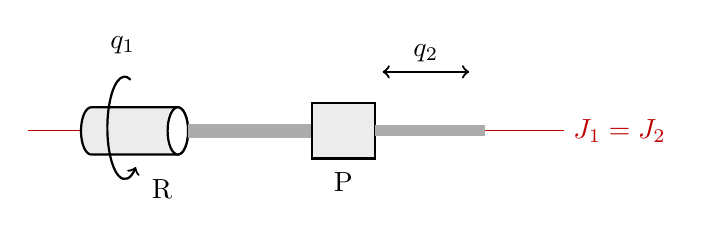
\begin{tikzpicture}
\draw[red!75!black] (-.8,0)--(6,0) node[right] {$J_1=J_2$};
\path[draw,thick,fill=gray!15] (0,-.3)--(1.1,-.3)
 arc[start angle=-90,end angle=90,x radius=.13,y radius=.3]
 --(0,.3) arc[start angle=90,end angle=270,x radius=.13,y radius=.3];
\draw[fill=white,thick] (1.1,0) ellipse (.13 and .3);
\draw[line width=5pt,gray!65] (1.23,0)--(2.8,0);
\draw[fill=gray!15,thick] (2.8,-.35) rectangle (3.6,.35);
\draw[line width=4pt,gray!65] (3.6,0)--(5,0);
\draw[<->,thick] (3.7,.75)--(4.8,.75) node[midway,above] {$q_2$};
\draw[->,thick] (.5,.65) arc[start angle=70,end angle=310,x radius=.22,y radius=.65];
\node[above] at (.4,.85) {$q_1$};
\node[below] at (.9,-.5) {R};
\node[below] at (3.2,-.4) {P};
\end{tikzpicture}

\caption{A revolute joint followed by a coaxial prismatic joint. Rotation
about the shared axis and translation along it are independent motions,
even though the two joint axes occupy the same line.}
\label{fig:l10-dh-coaxial}
\end{figure}

Coaxial R and P joints retain two independent coordinates, an angle and a
displacement. Two ideal coaxial R joints can also exist, but their
downstream orientation depends on the sum of their angles when the
positive directions agree. They are redundant for that downstream
kinematic effect; this does not make the two physical joints identical.

\subsection{Base and terminal frames}
Frame 0 has $z_0$ along $J_1$. Choose $O_0$ on that axis and choose a
perpendicular $x_0$. For a fixed base, this frame stays fixed while the
first moving link rotates. Aligning $x_0$ with a link in one configuration
does not make the first joint angle identically zero.

At the terminal link there is no physical $J_{n+1}$. Placing $O_n$ at
the tool point makes the final translation column directly useful.
The line through $O_n$ in the $x_n$ direction must intersect and be
perpendicular to $J_n$ for the standard DH construction. If $O_n$ is off
$J_n$, this selects the normal through that point. If $O_n$ is on $J_n$,
any perpendicular direction through it can be chosen. Then choose $z_n$
perpendicular to $x_n$; taking it parallel and equally directed to
$z_{n-1}$ often sets $\alpha_n=0$.

A required tool orientation need not obey these convenient choices.
In that case, retain a valid terminal DH frame and append the fixed tool
transformation. Changing a base or terminal frame changes the coordinates
reported by the model, even though the physical robot is the same.

\section{DH example: a planar RR arm}
\label{sec:l10-dh-rr}
Consider two revolute joints with parallel axes, followed by a tool at
the end of the second link. The link lengths are $\ell_1$ and $\ell_2$.
There are two joints, three frames, one common normal between the physical
joint axes, and two rows in the DH table.

\begin{figure}[htbp]
\centering\begin{tikzpicture}[scale=1.3]
\definecolor{dhbase}{RGB}{30,150,65}
\definecolor{dhone}{RGB}{155,65,180}
\definecolor{dhtool}{RGB}{225,115,20}
\coordinate (O) at (0,0);
\coordinate (A) at (3.35,.42);
\coordinate (B) at (4.95,2.22);
% Joint axes, selected common normal, and two alternative levels.
\draw[red!75!black] (-.3,-.81)--(.7,1.9) node[above] {$J_1$};
\draw[red!75!black] (3.05,-.39)--(4.05,2.32) node[above] {$J_2$};
\draw[sensorframe,dashed] (-.245,-.665)--(3.105,-.245);
\draw[sensorframe,dashed] (.455,1.235)--(3.805,1.655);
% Solid mechanical links, followed by the cylindrical joint bodies.
\draw[line width=9pt,gray!65] (O)--(A)--(B);
\draw[line width=6pt,gray!12] (O)--(A)--(B);
\foreach \p in {O,A} {
 \begin{scope}[shift={(\p)}]
 \path[draw,thick,fill=gray!15] (-.3,-.11)--(-.09,.46)
 arc[start angle=160,end angle=-20,x radius=.245,y radius=.12]
 --(.16,-.27) arc[start angle=-20,end angle=-200,x radius=.245,y radius=.12];
 \draw[fill=white,thick,rotate around={-20:(.12,.38)}] (.12,.38) ellipse (.245 and .12);
 \end{scope}
}
\draw[thick] ($(B)+(-.18,.05)$)--($(B)+(-.03,.35)$)--($(B)+(.13,.23)$);
\draw[thick] ($(B)+(.16,-.11)$)--($(B)+(.33,.17)$)--($(B)+(.18,.23)$);
\draw[sensorframe,thick] (O)--node[below,sloped] {$\mathrm{CN}_1$}(A);
\draw[axis,dhbase] (O)--(.35,.95) node[left] {$z_0$};
\draw[axis,dhbase] (O)--(1,-.22) node[below right] {$x_0$};
\draw[axis,dhone] (A)--++(.35,.95) node[left] {$z_1$};
\draw[axis,dhone] (A)--++(1.1,.138) node[right] {$x_1$};
\draw[axis,dhtool] (B)--++(.35,.95) node[above left] {$z_2$};
\draw[axis,dhtool] (B)--++(.8,.9) node[right] {$x_2$};
\foreach \p in {O,A,B} {\fill (\p) circle (.035);}
\node[dhbase,left] at (O) {$O_0$};
\node[dhone,below] at ($(A)+(0,-.18)$) {$O_1$};
\node[dhtool,below right] at (B) {$O_2$};
\draw[<->] (.1,.84)--node[above,sloped] {$\ell_1$}(3.45,1.26);
\draw[<->] (4.9,.12)--node[below right] {$\ell_2$}(6.5,1.92);
\draw[projection] (O)--(1.25,.156);
\draw[->,red!75!black] (.72,-.158) .. controls (.85,-.12) and (.87,.02) .. (.82,.103);
\node[red!75!black] at (1.08,.03) {$q_1$};
\draw[projection] (A)--++(1.4,.175);
\draw[->,red!75!black] ($(A)+(.9,.113)$) .. controls (4.25,.8) and (4.04,.99) .. (3.91,1.05);
\node[red!75!black] at (4.35,1.03) {$q_2$};
\end{tikzpicture}

\caption{Perspective view of the planar RR arm, with cylindrical revolute
joints and the terminal tool. The selected common normal follows the
first link. Dashed alternatives illustrate the freedom to shift it along
the parallel axes. Frame 0 is fixed; frames 1 and 2 move with their links.}
\label{fig:l10-dh-rr}
\end{figure}

Choose $O_0$ at the first joint and $O_1$ at the second, at the same axial
level. Put $O_2$ at the tool point. Let all three $z$ axes point in the
same direction, normal to the plane of motion. Choose $x_1$ along the
first link toward the second joint, and $x_2$ along the second link toward
the tool. The fixed $x_0$ defines the zero of $q_1$.

With the joint zeros chosen to match the DH angles, $\theta_1=q_1$ and
$\theta_2=q_2$. The second angle is measured relative to the first link,
not relative to the base. Since the $z$ axes are equally directed and
there is no displacement along them, the table is
\begin{center}
\begin{tabular}{ccccc}
\toprule
$i$ & $\theta_i$ & $\alpha_i$ & $a_i$ & $d_i$\\
\midrule
1 & $q_1$ & $0$ & $\ell_1$ & $0$\\
2 & $q_2$ & $0$ & $\ell_2$ & $0$\\
\bottomrule
\end{tabular}
\end{center}
The column order is a presentation choice; the column labels determine
the meaning. The joint count determines the number of rows. Filling the
variable entries first helps prevent mistaking an angle that happens to
be zero in the drawing for a constant zero parameter.

\subsection{Local matrices and the complete product}
Write $c_i=\cos q_i$, $s_i=\sin q_i$,
$c_{12}=\cos(q_1+q_2)$, and $s_{12}=\sin(q_1+q_2)$.
Each local matrix is a $z$ rotation followed by a translation along the
rotated $x$ axis:
\[
 H_1^0=\begin{bmatrix}
 c_1&-s_1&0&\ell_1c_1\\s_1&c_1&0&\ell_1s_1\\
 0&0&1&0\\0&0&0&1
 \end{bmatrix},\qquad
 H_2^1=\begin{bmatrix}
 c_2&-s_2&0&\ell_2c_2\\s_2&c_2&0&\ell_2s_2\\
 0&0&1&0\\0&0&0&1
 \end{bmatrix}.
\]
Their product is
\begin{equation}
 H_2^0=\begin{bmatrix}
 c_{12}&-s_{12}&0&\ell_1c_1+\ell_2c_{12}\\
 s_{12}&c_{12}&0&\ell_1s_1+\ell_2s_{12}\\
 0&0&1&0\\0&0&0&1
 \end{bmatrix}.
 \label{eq:l10-dh-rr}
\end{equation}
The translation column reproduces the geometric result in
Equation~\eqref{eq:l10-planar}, and the tool yaw is $q_1+q_2$.
DH has provided a systematic route to the same answer.

As a quick check, with $\ell_1=1\,\mathrm m$, $\ell_2=0.5\,\mathrm m$,
$q_1=0$, and $q_2=\pi/2$, the tool is at
$(1,0.5,0)\,\mathrm m$ and its $x_2$ axis points along $y_0$.
At $q_1=q_2=0$, the arm extends along $x_0$ to
$(\ell_1+\ell_2,0,0)$.

\section{DH example: a spatial RRP arm}
\label{sec:l10-dh-rrp}
The next arm has two revolute joints and one prismatic joint. The first
axis is vertical. The second intersects it at a height $\ell_1$ and is
perpendicular to it. The prismatic axis intersects the second joint axis
at a distance $\ell_2$ along that axis. The tool moves along the prismatic
axis. These are three joints and require four frames and three DH rows.

\begin{figure}[htbp]
\centering\begin{tikzpicture}[scale=1.3]
\definecolor{dhbase}{RGB}{30,150,65}
\definecolor{dhone}{RGB}{225,115,20}
\definecolor{dhtwo}{RGB}{155,65,180}
\definecolor{dhthree}{RGB}{195,65,120}
% Consistent oblique projection: X=(1,.1), Y=(-.8,.4), Z=(0,1).
% Shown at q1=pi, q2=0, l1=3, l2=3.5, q3=1.5 (drawing units).
\coordinate (O) at (0,0);
\coordinate (A) at (0,3);
\coordinate (B) at (2.8,1.6);
\coordinate (T) at (2.8,3.1);
\draw[red!75!black] (0,-.3)--(0,4.1) node[above] {$J_1$};
\draw[red!75!black] (-1.2,3.6)--(3.8,1.1) node[right] {$J_2$};
\draw[red!75!black] (2.8,.6)--(2.8,4.1) node[above] {$J_3$};
% Base revolute joint and upright support.
\draw[line width=6pt,gray!60] (0,.4)--(A);
\path[draw,thick,fill=gray!15] (-.35,.9)--(-.35,1.8)
 arc[start angle=180,end angle=0,x radius=.35,y radius=.12]
 --(.35,.9) arc[start angle=0,end angle=-180,x radius=.35,y radius=.12];
\draw[fill=white,thick] (0,1.8) ellipse (.35 and .12);
% Second revolute joint and its link toward the slider assembly.
\draw[line width=8pt,gray!70] (A)--(B);
\draw[line width=5pt,gray!15] (A)--(B);
\begin{scope}[shift={(A)},rotate=-26.565]
\path[draw,thick,fill=gray!15] (-.45,-.23)--(.55,-.23)
 arc[start angle=-90,end angle=90,x radius=.12,y radius=.23]
 --(-.45,.23) arc[start angle=90,end angle=270,x radius=.12,y radius=.23];
\draw[fill=white,thick] (.55,0) ellipse (.12 and .23);
\end{scope}
% Prismatic block, shaft, and terminal gripper.
\path[draw,thick,fill=gray!15] (2.45,1.25)--(3.05,1.15)--(3.05,1.8)--(2.45,1.9)--cycle;
\path[draw,thick,fill=white] (2.45,1.9)--(2.72,2.1)--(3.32,2)--(3.05,1.8)--cycle;
\path[draw,thick,fill=gray!30] (3.05,1.15)--(3.32,1.35)--(3.32,2)--(3.05,1.8)--cycle;
\draw[line width=5pt,gray!70] (B)--(T);
\draw[thick] (2.55,3.1)--(2.6,3.4)--(2.72,3.25);
\draw[thick] (3.05,3.1)--(3,3.4)--(2.88,3.25);
\draw[<->,thick] (3.65,1.85)--(3.65,2.65) node[midway,right] {P};
% Common normals through the intersecting joint axes.
\draw[sensorframe] (-1.25,2.875)--(1.05,3.105);
\node[sensorframe,above] at (1.05,3.2) {$\mathrm{CN}_1$};
\draw[sensorframe] (1.5,1.47)--(4.05,1.725) node[right] {$\mathrm{CN}_2$};
\draw[axis,dhbase] (O)--(0,.65) node[below left] {$z_0$};
\draw[axis,dhbase] (O)--(1.3,.13) node[right] {$x_0$};
\draw[axis,dhone] (A)--++(-1,-.1) node[below] {$x_1$};
\draw[axis,dhone] (A)--++(.8,-.4) node[below] {$z_1$};
\draw[axis,dhtwo] (B)--++(-1,-.1) node[left] {$x_2$};
\draw[axis,dhtwo] (B)--++(0,.95) node[left] {$z_2$};
\draw[axis,dhthree] (T)--++(-1,-.1) node[left] {$x_3$};
\draw[axis,dhthree] (T)--++(0,.7) node[left] {$z_3$};
\foreach \p in {O,A,B,T} {\fill (\p) circle (.035);}
\node[dhbase,below left] at (O) {$O_0$};
\node[dhone,above left] at (A) {$O_1$};
\node[dhtwo,below left] at (B) {$O_2$};
\node[dhthree,right] at (T) {$O_3$};
\draw[<->] (-1.7,0)--node[left] {$\ell_1$}(-1.7,3);
\draw[projection] (O)--(-1.8,0);
\draw[projection] (A)--(-1.8,3);
\draw[<->] (.2,4.25)--node[above,sloped] {$\ell_2$}(3,2.85);
\draw[projection] (A)--(.2,4.25);
\draw[projection] (B)--(3,2.85);
\draw[<->] (4.35,1.6)--node[right] {$q_3$}(4.35,3.1);
\draw[projection] (B)--(4.45,1.6);
\draw[projection] (T)--(4.45,3.1);
\end{tikzpicture}

\caption{The spatial RRP arm. The two cylinders represent revolute joints;
the block and sliding shaft represent the prismatic joint. Both neighboring
joint-axis pairs intersect, so their common normals pass through the
intersections. This illustrative configuration has $q_1=\pi$, $q_2=0$,
and $q_3>0$: the prismatic axis is vertical here but tilts when joint 2
rotates. Frames use distinct colors for readability.}
\label{fig:l10-dh-rrp}
\end{figure}

\subsection{Frames, signs, and the DH table}
Place frame 0 below the intersection of $J_1$ and $J_2$, with $z_0$
upward. Put $O_1$ at that intersection and choose $z_1$ along $J_2$
toward the prismatic assembly. Put $O_2$ where $J_2$ meets $J_3$, with
$z_2$ along the positive prismatic motion. Finally, put $O_3$ at the tool,
with $z_3=z_2$ and $x_3=x_2$ in direction.

At each intersection, choose the common-normal sense so that the twists
are $\alpha_1=-\pi/2$ and $\alpha_2=+\pi/2$. The first is the rotation
from $z_0$ to $z_1$ about $x_1$; the second is from $z_1$ to $z_2$ about
$x_2$. Both have magnitude $90^\circ$, but their signs differ. Use the
right-hand rule around the named positive $x$ axis, rather than the
apparent angle on the page.

Because the joint axes intersect, $a_1=a_2=0$. The tool origin lies on
the prismatic axis, so $a_3=0$ too. These zeros do not mean that the
physical links have zero length: $\ell_1$ and $\ell_2$ enter as offsets
along $z_0$ and $z_1$. Define $q_3$ as the signed tool displacement from
$O_2$ along $z_2$, with no additional zero offset. Then
\begin{center}
\begin{tabular}{cccccc}
\toprule
$i$ & Type & $\theta_i$ & $\alpha_i$ & $a_i$ & $d_i$\\
\midrule
1 & R & $q_1$ & $-\pi/2$ & $0$ & $\ell_1$\\
2 & R & $q_2$ & $+\pi/2$ & $0$ & $\ell_2$\\
3 & P & $0$ & $0$ & $0$ & $q_3$\\
\bottomrule
\end{tabular}
\end{center}
The revolute coordinates are angles; $q_3$ is a length. The last row has
$\theta_3=0$ because the terminal axes have been aligned with frame 2,
not because the third joint is absent.

\subsection{Local transformations}
Using $c_i=\cos q_i$ and $s_i=\sin q_i$ for $i=1,2$, the three matrices are
\begin{align}
 H_1^0&=\begin{bmatrix}
 c_1&0&-s_1&0\\s_1&0&c_1&0\\0&-1&0&\ell_1\\0&0&0&1
 \end{bmatrix},\\
 H_2^1&=\begin{bmatrix}
 c_2&0&s_2&0\\s_2&0&-c_2&0\\0&1&0&\ell_2\\0&0&0&1
 \end{bmatrix},\\
 H_3^2&=\begin{bmatrix}
 1&0&0&0\\0&1&0&0\\0&0&1&q_3\\0&0&0&1
 \end{bmatrix}.
\end{align}
The last matrix is a pure translation. Increasing $q_3$ moves the tool
along $z_2$ without changing its orientation relative to link 2.

\subsection{Complete direct kinematics and geometric checks}
Multiplication yields
\begin{equation}
 H_3^0=\begin{bmatrix}
 c_1c_2&-s_1&c_1s_2&-\ell_2s_1+q_3c_1s_2\\
 s_1c_2&c_1&s_1s_2&\ell_2c_1+q_3s_1s_2\\
 -s_2&0&c_2&\ell_1+q_3c_2\\
 0&0&0&1
 \end{bmatrix}.
 \label{eq:l10-dh-rrp}
\end{equation}
Its translation can also be assembled as three physical displacements,
all expressed in frame 0:
\begin{equation}
 p_3^0=
 \ell_1\begin{bmatrix}0\\0\\1\end{bmatrix}
 +\ell_2\begin{bmatrix}-s_1\\c_1\\0\end{bmatrix}
 +q_3\begin{bmatrix}c_1s_2\\s_1s_2\\c_2\end{bmatrix}.
 \label{eq:l10-dh-rrp-position}
\end{equation}
The middle vector follows the second joint axis. Rotation about that
axis changes the prismatic direction but does not change the position
of $O_2$, which lies on the rotation axis itself. The final unit vector
is also the third column of $R_3^0$, the tool's $z$ direction.

For $q_2=0$, the prismatic direction is vertical and
\[
 p_3^0=\begin{bmatrix}-\ell_2\sin q_1\\
 \ell_2\cos q_1\\\ell_1+q_3\end{bmatrix}.
\]
For $q_2=\pi/2$, it is horizontal, so changing $q_3$ leaves the tool
height equal to $\ell_1$. These limiting cases check both the signs and
the assignment of the prismatic coordinate.

For example, let $\ell_1=0.6\,\mathrm m$, $\ell_2=0.4\,\mathrm m$,
$q_1=0$, $q_2=\pi/2$, and $q_3=0.3\,\mathrm m$. Then
\[
 H_3^0=\begin{bmatrix}
 0&0&1&0.3\\0&1&0&0.4\\-1&0&0&0.6\\0&0&0&1
 \end{bmatrix}.
\]
The tool is at $(0.3,0.4,0.6)\,\mathrm m$ and its positive $z_3$
direction is $+x_0$. Increasing the extension by $0.1\,\mathrm m$
therefore increases only its $x_0$ coordinate by $0.1\,\mathrm m$.

\subsection{Checking a completed DH model}
A useful check is to distinguish geometry constants from joint variables.
An axis alignment visible in one drawing may disappear when a joint
moves. Conversely, the twist between adjacent joint axes is a fixed
property of the intervening rigid link in these models.

Check that there is one table row per joint, that each row contains the
correct variable parameter, and that translations are signed projections.
Then test a simple configuration against the robot drawing. If a different
valid frame assignment gives a different table, compare the resulting
poses only after expressing them in the same base and tool frames and
accounting for any changes in the joint zeros or positive directions.


\clearpage
\section{Additional exercises}
\subsection{Arm kinematics and workspace}
Assume ideal rigid links, independent joints, and no joint limits or
collisions unless stated otherwise.
\begin{enumerate}
\item \textbf{Joint descriptions.} An RPR arm has a fixed base. State its
number of configuration degrees of freedom, which links each joint connects,
and the units of each component of $q$. Explain why the letters RPR alone
are insufficient to compute the tool pose.

\item \textbf{Local versus world pose.} In a five-joint serial arm, hold
$q_2$ fixed and change $q_1$. Which of $H_2^1$ and $H_2^0$ can change?
Repeat the question when only $q_4$ changes. Explain your answers physically.

\item \textbf{Transform composition.} Write $H_{\mathrm{EE}}^W$ for a
three-joint arm with a nonidentity base transform $H_0^W$ and a fixed tool
transform $H_{\mathrm{EE}}^3$. State the mapping direction of each factor
and explain why inverting the result does not solve inverse kinematics.

\item \textbf{Planar direct kinematics.} Let $\ell_1=1\,\mathrm m$,
$\ell_2=0.5\,\mathrm m$, $q_1=\pi/2$, and $q_2=-\pi/2$. Compute the
tip position, yaw, and planar homogeneous matrix. Verify the result by
multiplying $H_1^0H_2^1$.

\item \textbf{Workspace and orientation.} For the same link lengths,
decide whether positions $(2,0)$, $(0.2,0)$, and $(1,0)$ in meters are
reachable. If the tip is at $(1.5,0)$, can its yaw be $\pi/2$? Explain
using the fully extended configuration.

\item \textbf{Two inverse solutions.} For $\ell_1=\ell_2=1\,\mathrm m$,
substitute $(q_1,q_2)=(0,\pi/2)$ and $(\pi/2,-\pi/2)$ into the forward
equations. Compare their positions and orientations. Which solution meets
the full target pose $(x,y,\psi)=(1,1,0)$?

\item \textbf{Task-dependent redundancy.} Compare planar arms with two,
three, and six independent revolute joints for a position-only task and
for a full planar-pose task. Assume generic nonsingular configurations.
Explain why an arm with two independently driven joints is not necessarily
underactuated, even though it cannot set an arbitrary planar tool pose.
\end{enumerate}

\clearpage
\subsection{DH frames and transformations}
\begin{enumerate}
\item \textbf{Indices and frame counts.} A fixed-base arm has five
one-degree-of-freedom joints. How many link frames, physical joint axes,
common normals between consecutive physical axes, and DH table rows are
needed? Which joint acts about or along $z_2$? Explain why $z_5$ does not
imply a sixth joint.

\item \textbf{Signed displacements.} A DH construction has
$\overrightarrow{O_{i-1}O_i}=-0.2\hat z_{i-1}+0.5\hat x_i$ in meters.
Find $d_i$, $a_i$, and the distance between the origins. Explain why the
negative value is compatible with a valid frame assignment.

\item \textbf{Deriving the local matrix.} Multiply
Equations~\eqref{eq:l10-dh-z} and~\eqref{eq:l10-dh-x} explicitly.
Explain why the translation column contains $a_i\cos\theta_i$ and
$a_i\sin\theta_i$, even though the second factor translates only along
its own $x$ axis.

\item \textbf{A revolute DH row.} Let $a_i=0.2\,\mathrm m$,
$d_i=0.1\,\mathrm m$, $\alpha_i=-\pi/2$, and
$\theta_i=q_i+\pi/2$. Compute $H_i^{i-1}$ at $q_i=0$.
Read the origin and all three axis directions from your answer, and
verify that the rotation is right-handed.

\item \textbf{A prismatic DH row.} Let $a_i=0.3\,\mathrm m$,
$\alpha_i=0$, $\theta_i=\pi/2$, and $d_i=q_i+0.1\,\mathrm m$.
Compute $H_i^{i-1}$ for $q_i=0.2\,\mathrm m$ and $0.4\,\mathrm m$.
Which entries change? Express the displacement between these configurations
in frame $i-1$.

\item \textbf{Recovering the planar arm.} Build a two-row DH table for
the planar RR arm using the parameter choices at the end of
Section~\ref{sec:l10-dh-procedure}. Multiply the spatial matrices and
recover Equation~\eqref{eq:l10-planar}. Identify the final $z$ direction.

\item \textbf{Consistency of conventions.} Explain why reversing a
chosen joint-axis direction while leaving every parameter and encoder
sign unchanged generally changes the predicted motion. Why can two
different DH tables nevertheless model the same physical arm?
\end{enumerate}

\clearpage
\subsection{DH examples and special cases}
\begin{enumerate}
\item \textbf{Parallel axes.} Explain why two distinct parallel joint
axes have infinitely many common normals. For a planar RR arm, describe
a choice that gives $d_1=0$. Why must the frames stay fixed to their links
after making this choice?

\item \textbf{Intersecting axes.} At an intersection, let
$\hat z_{i-1}=(0,0,1)$ and $\hat z_i=(0,1,0)$ in a common right-handed
frame. Choose $\hat x_i=(1,0,0)$. Find $a_i$ and the signed twist
$\alpha_i$. Repeat with $\hat x_i=(-1,0,0)$. Is an arbitrary direction
through the intersection an admissible $x_i$ axis?

\item \textbf{Planar RR calculation.} Use the DH table in
Section~\ref{sec:l10-dh-rr} with $\ell_1=0.8\,\mathrm m$,
$\ell_2=0.4\,\mathrm m$, $q_1=\pi/2$, and $q_2=-\pi/2$.
Compute $H_2^0$ and verify its translation by drawing the two link vectors.

\item \textbf{Spatial RRP calculation.} For the table in
Section~\ref{sec:l10-dh-rrp}, take $\ell_1=0.6\,\mathrm m$,
$\ell_2=0.4\,\mathrm m$, $q_1=\pi/2$, $q_2=\pi/2$, and
$q_3=0.3\,\mathrm m$. Compute the tool position and rotation matrix.
In which base-frame direction does the tool move if $q_3$ increases?

\item \textbf{A vertical configuration is not a fixed constraint.}
For the same RRP arm, hold $q_1$ and $q_3$ fixed and compare $q_2=0$
with $q_2=\pi/2$. Find the tool height and prismatic direction in each
case. Explain why $a_1=a_2=a_3=0$ does not imply a robot of zero size.

\item \textbf{Moving the base origin.} Place a new base origin at $O_1$
of the RRP arm, keeping its axes parallel to the old base axes and fixed
in space. Which DH constant becomes zero? Write the fixed transformation
that restores the tool pose relative to the original base.

\item \textbf{Coaxial joints.} For an ideal coaxial RP chain, choose
$a_1=a_2=0$, $\alpha_1=\alpha_2=0$, $d_1=0$, $\theta_1=q_1$,
$\theta_2=0$, and $d_2=q_2$. Compute $H_2^0$. Explain why both coordinates
affect the tool pose. How does this differ from two coaxial revolute
joints with zero axial offsets?
\end{enumerate}
